% This file was created by matplotlib2tikz v0.6.14.
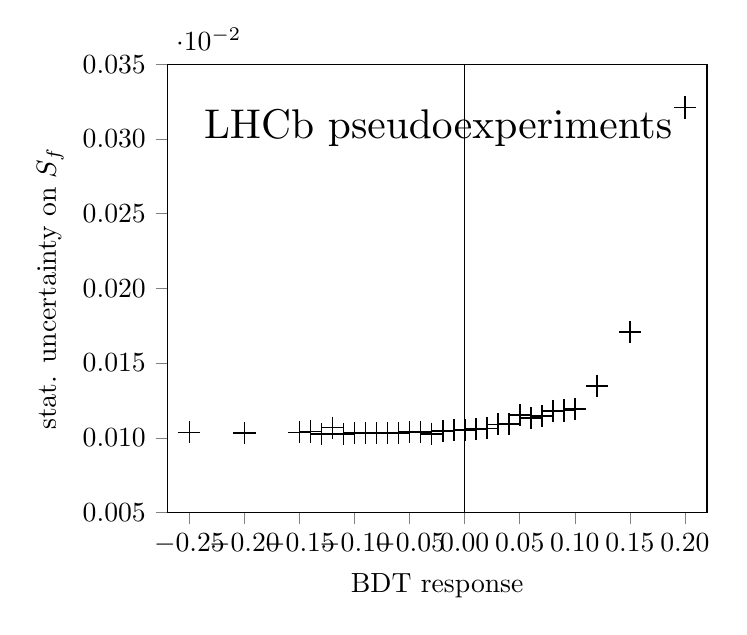
\begin{tikzpicture}

\begin{axis}[
xlabel={BDT response},
ylabel={stat. uncertainty on $S_{f}$},
xmin=-0.27, xmax=0.22,
ymin=0.005, ymax=0.035,
xtick={-0.3,-0.25,-0.2,-0.15,-0.1,-0.05,5.55111512312578e-17,0.05,0.1,0.15,0.2,0.25},
xticklabels={,$-0.25$,$-0.20$,$-0.15$,$-0.10$,$-0.05$,$0.00$,$0.05$,$0.10$,$0.15$,$0.20$,},
ytick={0,0.005,0.01,0.015,0.02,0.025,0.03,0.035,0.04},
yticklabels={,$0.005$,$0.010$,$0.015$,$0.020$,$0.025$,$0.030$,$0.035$,},
tick align=outside,
tick pos=left,
x grid style={white!69.019607843137251!black},
y grid style={white!69.019607843137251!black}
]
\path [draw=black, semithick] (axis cs:-0.25,0.0102973603896932)
--(axis cs:-0.25,0.0104246396103068);

\path [draw=black, semithick] (axis cs:-0.2,0.0102976507575951)
--(axis cs:-0.2,0.0103273492424049);

\path [draw=black, semithick] (axis cs:-0.15,0.0103107096320981)
--(axis cs:-0.15,0.0104082903679019);

\path [draw=black, semithick] (axis cs:-0.14,0.0104072720779386)
--(axis cs:-0.14,0.0104327279220614);

\path [draw=black, semithick] (axis cs:-0.13,0.0101970527778486)
--(axis cs:-0.13,0.0103059472221514);

\path [draw=black, semithick] (axis cs:-0.12,0.010659408116908)
--(axis cs:-0.12,0.010697591883092);

\path [draw=black, semithick] (axis cs:-0.11,0.0102012954185358)
--(axis cs:-0.11,0.0103017045814642);

\path [draw=black, semithick] (axis cs:-0.1,0.0102686446609407)
--(axis cs:-0.1,0.0103393553390593);

\path [draw=black, semithick] (axis cs:-0.09,0.0103278578643763)
--(axis cs:-0.09,0.0103561421356237);

\path [draw=black, semithick] (axis cs:-0.08,0.0103039289321881)
--(axis cs:-0.08,0.0103180710678119);

\path [draw=black, semithick] (axis cs:-0.07,0.0103137218254069)
--(axis cs:-0.07,0.0103292781745931);

\path [draw=black, semithick] (axis cs:-0.06,0.010218655808229)
--(axis cs:-0.06,0.010446344191771);

\path [draw=black, semithick] (axis cs:-0.05,0.0103424020202536)
--(axis cs:-0.05,0.0104215979797464);

\path [draw=black, semithick] (axis cs:-0.04,0.0103597867965644)
--(axis cs:-0.04,0.0104022132034356);

\path [draw=black, semithick] (axis cs:-0.03,0.0102479583694397)
--(axis cs:-0.03,0.0102960416305603);

\path [draw=black, semithick] (axis cs:-0.02,0.010441372583002)
--(axis cs:-0.02,0.010486627416998);

\path [draw=black, semithick] (axis cs:-0.01,0.0104840649711575)
--(axis cs:-0.01,0.0105109350288425);

\path [draw=black, semithick] (axis cs:0,0.0104901299423149)
--(axis cs:0,0.0105438700576851);

\path [draw=black, semithick] (axis cs:0.01,0.0105611360389693)
--(axis cs:0.01,0.0105738639610307);

\path [draw=black, semithick] (axis cs:0.02,0.0105950233405971)
--(axis cs:0.02,0.0106699766594029);

\path [draw=black, semithick] (axis cs:0.03,0.0108921715728753)
--(axis cs:0.03,0.0108978284271247);

\path [draw=black, semithick] (axis cs:0.04,0.0108031055556973)
--(axis cs:0.04,0.0110208944443027);

\path [draw=black, semithick] (axis cs:0.05,0.0114656091270347)
--(axis cs:0.05,0.0115433908729653);

\path [draw=black, semithick] (axis cs:0.06,0.0113054791847198)
--(axis cs:0.06,0.0113295208152802);

\path [draw=black, semithick] (axis cs:0.07,0.01142078069991)
--(axis cs:0.07,0.01150421930009);

\path [draw=black, semithick] (axis cs:0.08,0.01181)
--(axis cs:0.08,0.01181);

\path [draw=black, semithick] (axis cs:0.09,0.0118157218254069)
--(axis cs:0.09,0.0118312781745931);

\path [draw=black, semithick] (axis cs:0.1,0.0118905025253169)
--(axis cs:0.1,0.0119894974746831);

\path [draw=black, semithick] (axis cs:0.12,0.0134698578643763)
--(axis cs:0.12,0.0134981421356237);

\path [draw=black, semithick] (axis cs:0.15,0.0170544730880654)
--(axis cs:0.15,0.0171195269119346);

\path [draw=black, semithick] (axis cs:0.2,0.0320527096320981)
--(axis cs:0.2,0.0321502903679019);

\addplot [semithick, black, mark=+, mark size=4, mark options={solid}, only marks, forget plot]
table {%
-0.25 0.010361
-0.2 0.0103125
-0.15 0.0103595
-0.14 0.01042
-0.13 0.0102515
-0.12 0.0106785
-0.11 0.0102515
-0.1 0.010304
-0.09 0.010342
-0.08 0.010311
-0.07 0.0103215
-0.06 0.0103325
-0.05 0.010382
-0.04 0.010381
-0.03 0.010272
-0.02 0.010464
-0.01 0.0104975
0 0.010517
0.01 0.0105675
0.02 0.0106325
0.03 0.010895
0.04 0.010912
0.05 0.0115045
0.06 0.0113175
0.07 0.0114625
0.08 0.01181
0.09 0.0118235
0.1 0.01194
0.12 0.013484
0.15 0.017087
0.2 0.0321015
};
\path [draw=black, fill opacity=0] (axis cs:0,0.005)
--(axis cs:0,0.035);

\path [draw=black, fill opacity=0] (axis cs:1,0.005)
--(axis cs:1,0.035);

\path [draw=black, fill opacity=0] (axis cs:-0.27,0)
--(axis cs:0.22,0);

\path [draw=black, fill opacity=0] (axis cs:-0.27,1)
--(axis cs:0.22,1);

\node at (axis cs:-0.25,0.03)[
  scale=1.5,
  anchor=base west,
  text=black,
  rotate=0.0
]{ LHCb pseudoexperiments};
\end{axis}

\end{tikzpicture}